\subsection{曲面立体}
曲面体是由面或曲面和平面共同构成的立体,其中最常见的是回转曲面。回转体曲面是由一母线绕一空间轴线作旋转运动而形成的光滑曲面。母线在在回转曲面上任意位置称作素线,母线上任意一点的旋转轨迹都是一个圆,该圆称为纬圆。图\ref{fig:huizhuangti}所示为回转体的形成和术语。
\begin{figure}[htbp]
\centering
\subfloat[]{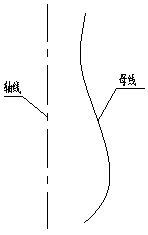
\includegraphics[scale=0.5]{huizhuangti.png}}\hspace{30pt}
\subfloat[]{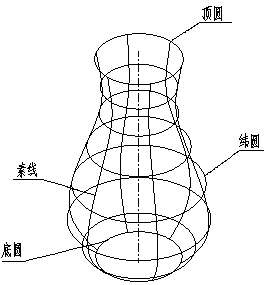
\includegraphics[scale=0.5]{rotatetree.png}}
\caption{回转体的形成及术语}\label{fig:huizhuangti}
\end{figure}

画回转体的投影图时,首先画出回转轴线,然后画出反映实形的投影,最后画其余两个投影。回转曲面向某一投影面投影时,轮廓素线是回转曲面在该投影面上可见和不可见面的分界线的投影,在分界线之前的回转曲面为可见,反之则不可见。画图时,凡不属于该投影面的轮廓素线,一律不画出。
\subsubsection{圆柱体}
圆柱体是由圆柱面、顶面、底面所构成的。圆柱体可以看作一条与轴线平行的母线绕轴线旋转而成的。图所示圆柱体的轴线垂直于水平投影面,其水平投影为圆;其正投影和侧投影均为矩形。
\begin{figure}[htbp]
\centering
\subfloat[]{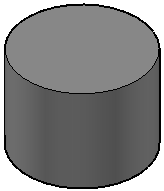
\includegraphics[scale=0.9]{yuanzhuti.png}}\hspace{30pt}
\subfloat[]{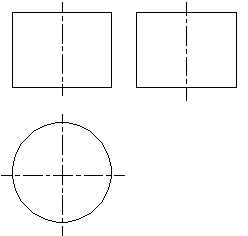
\includegraphics[scale=0.7]{yuanzhutithreeview.png}}
\caption{圆柱体的投影}\label{fig:yuanzhuti}
\end{figure}
\subsubsection{圆锥体}
图\ref{fig:yuanzhuiti} 所示的圆锥体底面与水平投影面平行,其投影为一圆,反映实形,在其余两个投影面上积聚为一条直线;圆锥体的其余两面投影均为等腰三角形。
\begin{figure}[htbp]
\centering
\subfloat[]{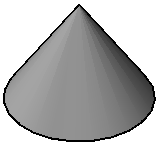
\includegraphics[scale=1]{yuanzhuiti.png}}\hspace{30pt}
\subfloat[]{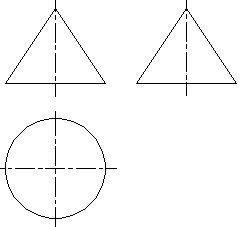
\includegraphics[scale=0.7]{yuanzhuitithreeview.png}}
\caption{圆锥体的投影}\label{fig:yuanzhuiti}
\end{figure}
\subsubsection{球体}
球体是由圆形母线以其直径为回转轴旋转而成的。球体的三面投影均为圆。
\begin{figure}[htbp]
\centering
\subfloat[]{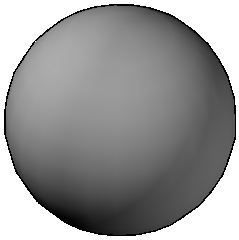
\includegraphics[scale=0.7]{qiouti.png}}\hspace{30pt}
\subfloat[]{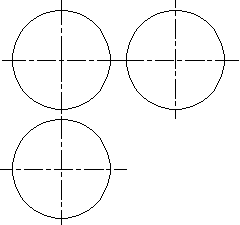
\includegraphics[scale=0.7]{qioutithreeview.png}}
\caption{球体的投影}\label{fig:qiout}
\end{figure}
\endinput